\documentclass[aps,prd,reprint,amsmath,amssymb,longbibliography,nofootinbib]{revtex4-2}
\usepackage[T1]{fontenc}
\usepackage{lmodern,xurl}
\usepackage{graphicx,booktabs,array,tabularx,xcolor}
\usepackage{hyperref}
\hypersetup{colorlinks=true,linkcolor=blue!45!black,citecolor=blue!45!black,urlcolor=blue!45!black}
\urlstyle{tt}
\newtheorem{theorem}{Theorem}
\newtheorem{proposition}[theorem]{Proposition}
\newtheorem{lemma}[theorem]{Lemma}
\newtheorem{corollary}[theorem]{Corollary}
\newcommand{\R}{\mathbb R}
\newcommand{\C}{\mathbb C}
\newcommand{\norm}[1]{\left\lVert #1\right\rVert}
\newcommand{\code}[1]{\texttt{#1}}
\newcommand{\baseline}{\code{3064d45}}
\newcommand{\auditpath}{\path{research/rigorous_performance_audit_20261027/}}
\begin{document}
\title{VigilODE: Adversarial Audit, Constructive Error Bounds,\texorpdfstring{\\}{ }and Measured Implementation Economy}
\author{VigilODE research audit}
\noaffiliation
\date{27 October 2026}
\begin{abstract}
We audit the latest available VigilODE checkpoint and profiling packet, separating adapter scheduling, integration kernels, and the mathematical obligations of structure-exploiting solvers. Previously completed repairs are treated as baseline facts. New production changes give incomplete comparisons their correct evidence type, optionally stop a dominated return comparator using conservative cost bounds, retain aligned dense-LU solve storage, eliminate an analytic partial-time-derivative temporary, and borrow projected matrix rows. Targeted native contracts pass 51 tests. With qualified numerical outputs, measured instruction counts decrease by 13.196\% for a 32-dimensional LU kernel, 2.605\% for a full 65-dimensional dense trajectory, and 1.731\% for a 16-dimensional adapter solve. Repeated wall and process-CPU timings remain too variable to establish reliable elapsed-time acceleration. We derive a minimax scalar relaxation for shifted dissipative systems, extend causal stage-error propagation to approximate inverses, and state the full-domain requirements for physical residual transport. The shifted-system research candidate satisfies all 27 finite operator checks but reaches the strict residual target in only 25 cases; it is not enabled as a solver default. An exact rational derivation separates ideal fixed-step DOPRI5 dispersion from an empirical adaptive tolerance law. None of these optimizations establishes an end-to-end physical certification of the separate V8 program.
\end{abstract}
\maketitle

\section{Scope and principal conclusions}
\label{sec:scope}
The inspected baseline is commit \path{3064d453091af1dec7f99f0c8afabd98b447ea34}, on the checkpoint-followup research branch. This supersedes the earlier integration snapshot \code{dda8d2f}. The profiling packet carried by this baseline measures source \code{46939bbe} on an AMD Ryzen 9 5900X; its wall-clock values are explicitly diagnostic. The current experiments use a different, shared Intel host. Historical measurements guide the choice of surfaces but are not relabeled as current performance results \cite{ProfilePacket,CheckpointPacket,IntegrationPacket}.

Three conclusions organize this audit. First, the sources do not establish a fundamental inconsistency in the project's structural mathematics. They do identify mathematical premises that an optimization cannot supply: a valid operator relation throughout a tube, inverse-action or propagation bounds, and control of reconstruction in the physical norm. Second, several costs are independent of those premises. Reallocating an unchanged stage RHS, copying a row before its dot product, and continuing an already dominated comparison are avoidable implementation costs. Third, the two classes of evidence must remain separate. Fewer work units do not prove lower wall time; a passing local error test does not certify global physical error; a contraction theorem does not prove that an iteration is economical.

\paragraph{Measured outcome.}
The warmed retained-LU solve adds zero allocations in the seven-size contract
cohort. The adapter removes 17 of 2119 and 50 of 2655 charged work units in the
8- and 16-dimensional fixtures, respectively, with exactly equal accepted
trajectories. All three dense fixtures likewise preserve every common observation
value and native counter. A separate Callgrind comparison measures instruction
reductions of 13.196\% for the 32-dimensional LU kernel, 2.605\% for the full
65-dimensional dense trajectory, and 1.731\% for the 16-dimensional adapter.
These establish implementation-work reductions in the profiled cohorts.
Wall-clock acceleration is \emph{not established}:
after an initial short-batch pass, a single longer confirmation gives paired
dense baseline/candidate ratios 1.033, 0.923 at dimensions 65 and 192 and
an adapter ratio 0.980 at dimension 16, but every observed block range
crosses unity. Process CPU ratios are also variable. Ratios above one favor
the candidate; neither attractive medians nor lower work counts are promoted
to reliable time-speedup claims. The shifted-factor research candidate is
excluded from production timing claims.


The work is performed in an isolated branch. Existing V6/V8 physical ledgers and previously closed campaigns are preserved. The V8 represented-query membership results remain scoped results: the retained delivery records do not claim a uniform whole-domain rounding bound, an actual ODE tube enclosure, or a complete native physical restoration. Their central status remains 27/88, with global physical completion unspecified and L4 false. This audit neither reruns those physical campaigns nor increments that count \cite{V8Membership,V8Tube}.

\section{Critical reading of the existing evidence}
\label{sec:audit}
\subsection{What was already repaired}
The latest checkpoint already admits nonfatal incomplete return comparators through a cost lower bound, includes an implicit-first return sentinel, preserves a productive implicit replay, and incorporates earlier derivative fallback and small-interval fixes. The prior approximately 90-to-3 allocations per matrix-free attempt reduction is also historical work. Claiming any of these as newly fixed would overstate the present contribution. Our adapter contribution is an earlier stopping point, conservative numerical evaluation of the sufficient inequality, and truthful evidence semantics.

\subsection{Where the measured time goes}
The old packet reports that discarded entry pilots account for 85\% and 80\% of the selector-minus-direct instruction excess on rotation and tight gyromotion, respectively. These apply to the opt-in \code{adaptive\_evidence(ProvidedOnly)} preset; the default switching configuration is DOPRI-only and runs no such pilots. These are adapter costs. Independently, matrix-free RODAS costs approximately 6.9 times the dense method's instructions in the small case5 controlled comparison. Its least-squares correction consumes 39\% of the transition-39 matrix-free instruction count, including 18\% in QR factorization. These are inner-mode costs. None of these historical percentages is a current timing measurement \cite{ProfilePacket}.

This distinction prevents two mistaken interventions. A faster LU solve cannot cure repeated losing entry pilots. Conversely, fewer selector probes do not fix the high cost of QR, orthogonalization, and operator construction inside a retained matrix-free step. The current dense-storage change applies to the Faer route, normally dimension above 64. The existing small-dense route was already optimized; it cannot receive credit for a new Faer improvement.

\begin{table*}[t]
\caption{Audit disposition. IDs refer to the 31-item latest profiling packet. ``Open'' means not established as resolved in this work; it does not imply that every proposed repair is necessary or valid.}
\label{tab:audit}
\centering\small
\begin{tabular}{@{}>{\raggedright\arraybackslash}p{0.12\textwidth} >{\raggedright\arraybackslash}p{0.23\textwidth} >{\raggedright\arraybackslash}p{0.59\textwidth}@{}}
\toprule
IDs & Surface & Disposition and justification \\
\midrule
A1 & Provenance/authority references & Historical missing-reference gates remain open. They are not evidence of a numerical theorem failing; no repository-wide promotion is claimed. \\
A2 & MF fresh-state allocation & Analytic supplied $f_t$ temporary removed. State copy/Arc construction and finite-difference $f_t$ remain. \\
A3--A4 & FD Jacobian and adapter allocation & Open. These require retained FD buffers and an explicit adapter storage contract. \\
A5 & Incomplete evidence semantics & Corrected: distinct lower-bound evidence, absent ratios for incomplete challengers, outward upper ratio for a completed winner versus a prefix. \\
A6, D3--D4 & Accuracy/output comparison & New dense tests use 33 common times; adapter checks every returned component and identical accepted trajectories. No continuous-supremum or universal WRMS certificate is inferred. \\
A7 & Gyromotion accuracy & Open physical requirement. A two-point empirical tolerance slope is separated from exact fixed-step dispersion in Sec.~\ref{sec:phase}. \\
B1, B3--B4, B7--B9, C9 & Probe scheduling/restarts & Repeated entry-pilot, horizon, seed, facade, and return-ramp costs remain open. New comparator stopping closes only a related, precisely specified return-comparison waste. \\
B2, B5, C1, C4 & Provider choice and cost proxy & Open coupled design question. No undeclared dense assembly replaces a JVP provider; no work-unit saving is treated as a time theorem. \\
B6, C2, C5 & Krylov kernels/wrappers & Open. QR/Givens substitution changes rounding, rank and breakdown semantics and is outside the exact-storage patch. \\
C3, C6--C8 & Records, controller, session, landing & Open; old instruction fractions are not portable release-build speedups. \\
D1--D2, D5--D6 & Measurement coverage & New raw paired timing, qualified errors, larger dense sizes, and a sentinel control improve this experiment. The old trace-tool defects and broad holdout coverage remain open. \\
New & Faer RHS and projected rows & Retained aligned solve storage and borrowed rows preserve the arithmetic path; separate tests and timings establish only the stated scope. \\
\bottomrule
\end{tabular}
\end{table*}

\subsection{Evidence defects that affect interpretation}
A completed candidate and a partly executed challenger are not two completed integrations. The previous telemetry nevertheless used a completed-comparison label and sometimes displayed a prefix/complete ratio as if it were a method-cost ratio. We correct this without treating a partial state as admissible output. A completed candidate divided by the challenger's lower-bound cost can be a conservative upper bound on its eventual ratio; a partly completed candidate divided by a completed incumbent is not the analogous comparison and now has no such ratio.

The profiling packet also admits endpoint-only accuracy in many rows, host-dependent timing classifications, and small cheap-RHS fixtures. Its reported gyromotion default error, approximately $3.16\times10^{-2}$ against a $10^{-4}$ cap, is not repaired by a faster selector. Its attribution to phase drift is a useful diagnostic, while its two-tolerance slope is insufficient to establish a universal law. Table~\ref{tab:audit} preserves unresolved findings instead of turning a finite optimization into a blanket closure.

% Body-only section for the parent's REVTeX report.
% Requires amsmath, amssymb; no theorem package or custom macros are required.
% Bibliography keys: TranquilliSandu2014, LiuMoursiVanderwerff2022.

\section{Mathematical audit and constructive repair}
\label{sec:theory-audit}

The audit separates a mathematical premise from the numerical evidence used to
instantiate it.  Exact carrier coordinates, polynomial resolvents, and finite
causal stage propagation are valid constructions under their declared
structure.  The present evidence does not establish a fundamental failure of
these ideas.  It does identify obligations that an allocation optimization
cannot discharge: the structure must hold on the relevant domain; a residual
must be transported through an inverse or flow-sensitivity bound; and the
result must refer to the original physical norm and requested outputs.
Conversely, temporary storage before an unchanged linear solve and continued
execution of a comparator whose cost has already lost are implementation or
scheduling costs.  Removing them does not require changing the integration
formula or its error threshold.

The distinction is relevant to the interpretation of the existing code.
The coupled solver explicitly labels its original-space residual as
operational rather than certified.  The causal-majorant implementation
contains finite triangular propagation and radius closure.  The conditioned
polynomial path binds a declared polynomial identity, coefficient defects,
and an original-operator residual.  These safeguards should be retained.
Classical Rosenbrock order conditions do not license arbitrary approximate
stage solves or an arbitrary replacement Jacobian; Rosenbrock--W and
Rosenbrock--K methods account for these approximations through their own order
theory.  This distinction is explicit in Sec.~1, following Eqs.~(2a)--(2b), of
Ref.~\cite{TranquilliSandu2014}.

\subsection{A partial-cost stopping theorem for the adapter}
\label{subsec:cost-theorem}

Fix an accepted checkpoint, a final time, an output contract, and an accuracy
qualification.  Both candidates use the same original state and cost units.
Let a completed explicit candidate satisfy this qualification at cost at most
$E$.  Let $L_k$ be the nondecreasing cost already spent by an implicit
comparator after its $k$th checked unit.  Every completion of that same
comparator must have a total cost $I\geq L_k$.  The native success flag supplies
the registered local-tolerance and output qualification; it does not by itself
supply a rigorous physical global-error bound.  If the stronger qualification
is required, it must be established separately.

\paragraph{Theorem 1 (prefix-cost dominance).}
For $0<\rho<1$, the condition
\begin{equation}
 E\leq \rho L_k
 \label{eq:prefix-dominance}
\end{equation}
implies $E\leq\rho I$ for every completion of the implicit comparator.  Hence
the explicit result may be selected, and the comparator may be stopped,
without computing its endpoint.  If the comparator does not complete, it
supplies no competing qualified result; the explicit result retains its
previously established qualification.

\paragraph{Proof.}
The monotonicity premise gives
$E\leq\rho L_k\leq\rho I$ for every comparator completion.  No state from the
incomplete comparator enters this inequality or the explicit result.
Numerical admissibility of the latter was established before the cost test.
\hfill$\square$

The latest baseline already uses the lower-bound argument for an incomplete
comparator.  The implementation refinement is to stop proactively once
Eq.~\eqref{eq:prefix-dominance} becomes decisive, use conservative scalar
arithmetic, and record evidence distinct from a completed same-window
comparison.  A callback-only lower bound is sufficient when all omitted
factorization, solve, and bookkeeping costs are nonnegative.  A count of
callbacks cannot be substituted for elapsed seconds in an inequality about
elapsed seconds.

In floating-point arithmetic, use an upper enclosure of $E$ and a lower
enclosure of $\rho L_k$.  With serial checking after a callback of maximum
weight $U$, a prescribed callback threshold $B$ permits charged work up to
$B+U$, together with any separately charged structural verification.  This is
a bound in the registered callback units, not a wall-clock bound.
An observed fatal callback remains terminal even when an explicit candidate
is available.  A typed cost stop must not conceal a fatal error.  Callback
replay must satisfy the caller's purity or transaction contract, and partial
implicit states are never committed.  The theorem compares the present
qualified observations; it does not guarantee future optimality or a fixed
fraction saved in the total solve, since candidate construction and discarded
work have already been paid.

\subsection{Uniformly convergent reuse of a dissipative shifted system}
\label{subsec:cayley-theorem}

Let $H$ be a finite-dimensional real or complex Hilbert space with a fixed
positive-definite metric $M$.  All norms and adjoints in this subsection refer
to this same metric.  A linear operator $J$ is assumed dissipative:
\begin{equation}
 \operatorname{Re}\langle v,Jv\rangle_M\leq0
 \quad\hbox{for every }v\in H.
 \label{eq:dissipativity}
\end{equation}
Negative real parts of eigenvalues alone are not this hypothesis.  Nor can a
state-dependent error metric be changed silently between the cached and
current systems.

Use the native scaled stage convention
\begin{equation}
 \begin{gathered}
 P=a_0^{-1}I-J,\qquad W=a^{-1}I-J,\\
 a_0>0,\quad a=\gamma h>0.
 \end{gathered}
 \label{eq:native-shifts}
\end{equation}
The shifts $a_0,a$ have units of time; $J,P,W$ have units of inverse time.
Set
\begin{equation}
 \omega_*={2a\over a+a_0},\qquad
 q_*={|a-a_0|\over a+a_0},\qquad
 R_0=(I-a_0J)^{-1}.
 \label{eq:optimal-relaxation}
\end{equation}

\paragraph{Theorem 2 (minimax scalar relaxation).}
Under Eq.~\eqref{eq:dissipativity}, both $P$ and $W$ are invertible.  The
iteration
\begin{equation}
 x_{k+1}=x_k+\omega_*P^{-1}(b-Wx_k)
 \label{eq:relaxed-richardson}
\end{equation}
contracts the error in the $M$ norm by at most $q_*<1$ for every positive shift
ratio.  Moreover, $\omega_*$ minimizes the uniform worst-case norm bound over
real scalar relaxations and all dissipative operators in this class.

\paragraph{Proof.}
If $Wv=0$, taking the real part of the inner product with $v$ gives
$a^{-1}\|v\|_M^2=\operatorname{Re}\langle v,Jv\rangle_M\leq0$, hence $v=0$.
Finite dimensionality implies invertibility.  The same reasoning applies to
$P$.

Write $v=(I-a_0J)u$.  Dissipativity gives
\begin{align}
 \|u+a_0Ju\|_M^2-\|u-a_0Ju\|_M^2
 &=4a_0\operatorname{Re}\langle u,Ju\rangle_M\nonumber\\
 &\leq0.
\end{align}
Therefore the reflected resolvent
\begin{equation}
 C=2R_0-I=(I+a_0J)(I-a_0J)^{-1}
\end{equation}
has norm at most one.  Put $s=a_0/a$.  Direct algebra yields
\begin{align}
 P^{-1}W
 &=I+(s-1)R_0\nonumber\\
 &={1+s\over2}I+{s-1\over2}C,
\end{align}
so the iteration matrix is exactly
\begin{equation}
 T_*=I-\omega_*P^{-1}W
 ={a-a_0\over a+a_0}C.
 \label{eq:cayley-iteration-identity}
\end{equation}
For $e_k=x_k-W^{-1}b$, one has $e_{k+1}=T_*e_k$, proving the contraction.

For minimax sharpness, the class contains $J=0$, for which the norm of the
iteration matrix with scalar relaxation $\omega$ is $|1-\omega s|$.  For the
family $J=-\lambda I$, its limit as $\lambda\to\infty$ is $|1-\omega|$.
Every uniform bound is therefore at least
\begin{equation}
 \max\{|1-\omega s|,|1-\omega|\}.
\end{equation}
Its minimum over real $\omega$ balances the two endpoint errors with opposite
signs, giving $\omega=2/(1+s)$ and value $|1-s|/(1+s)$.  Equation
\eqref{eq:cayley-iteration-identity} attains that uniform bound.
\hfill$\square$

The contraction of a reflected resolvent is a standard monotone-operator
fact, not a claimed novelty of this project.  Fact~2.5 and Eq.~(14) of
Ref.~\cite{LiuMoursiVanderwerff2022} state the corresponding equivalence; in
that convention the monotone operator is $A=-a_0J$.  The contribution here is
the explicit connection to the solver's scaled stage system and a bounded,
testable reuse candidate.  The existing lagged driver already has
Richardson, GMRES, and several staleness criteria.  Theorem~2 supplies an
additional metric-qualified candidate; it does not establish that this
candidate is faster than those existing choices.

\paragraph{Jacobian drift.}
Suppose the cached operator obeys
$\operatorname{Re}\langle v,J_0v\rangle_M\leq-\alpha\|v\|_M^2$ with
$\alpha\geq0$, while the current operator is $J=J_0+\Delta$.
Coercivity and Cauchy--Schwarz give
\begin{equation}
 \|P^{-1}\|_M\leq{a_0\over1+a_0\alpha}.
\end{equation}
Since the perturbed iteration matrix is
$T=T_*+\omega_*P^{-1}\Delta$,
\begin{equation}
 \|T\|_M\leq q_*+
 \omega_*{a_0\|\Delta\|_M\over1+a_0\alpha}=:q.
 \label{eq:cayley-drift}
\end{equation}
This derivation does not assume that $J_0$ and $\Delta$ commute.  A contraction
claim requires $q<1$ and a valid drift bound over the declared domain.

If the implemented inverse action is $\widehat R$, rather than exact
$P^{-1}$, and
$\|\widehat R-P^{-1}\|_M\leq\varepsilon_R$, the iteration also contains this
action error.  If the represented relaxation differs from the mathematical
value by at most $\varepsilon_\omega$, a sufficient additional allowance is
\begin{equation}
 \varepsilon_\omega\|P^{-1}W\|_M+
 |\widehat\omega|\varepsilon_R\|W\|_M.
 \label{eq:inverse-action-allowance}
\end{equation}
For fixed $J$, $\|P^{-1}W\|_M\leq\max(1,a_0/a)$.
A favorable observed residual ratio is not itself a full-space proof of
$\varepsilon_R$ or $q$.  Alternatively, use the iteration heuristically and
certify its final result by an independently valid original-target residual
bound.

\paragraph{Native residual units.}
If the actual $J$ has dissipation margin $\alpha'\geq0$, then for the original
scaled residual $r=b-Wx$,
\begin{equation}
 \|x-W^{-1}b\|_M
 \leq{a\over1+a\alpha'}\|r\|_M.
 \label{eq:scaled-residual-bound}
\end{equation}
Indeed, $\|W^{-1}\|_M\leq a/(1+a\alpha')$ follows from the same coercivity
argument.  Here $r$ has units of state per time.  The factor $a$ must not be
omitted or mixed with the normalized equation using $I-aJ$, whose residual
has state units.  The cached dissipation margin $\alpha$ in
Eq.~\eqref{eq:cayley-drift} and the actual-operator margin $\alpha'$ in
Eq.~\eqref{eq:scaled-residual-bound} are separate hypotheses.

\paragraph{Computational form and scope of verification.}
For $a\leq a_0$, compute $r=a/a_0$, then
\begin{equation}
 \omega_*={2r\over1+r},\qquad q_*={1-r\over1+r}.
\end{equation}
For $a>a_0$, compute $r=a_0/a$ and use $\omega_*=2/(1+r)$ with the same
expression for $q_*$.  This avoids overflow in $a+a_0$ and avoids a ratio
greater than one.  The research Rust primitive encloses the ratio, applies
the monotone formulas with outward scalar arithmetic, includes the
represented-$\omega$ allowance and declared drift, and refuses stale
model/metric/domain identities.  Its scalar argument assumes correctly
rounded basic binary64 operations, gradual underflow, and no
fast-math reassociation.  Tags prevent an identity mismatch; they do not
prove the truth of a caller declaration.  The primitive does not certify an
external floating-point LU action or residual callback, and it is not wired
into a production solver default.  Compilation with Rust 1.94.1 and all
seven targeted primitive tests succeeded.

The Python prototype used actual cached LU factors on 27 finite shifted
systems: diagonal dissipative, damped nonnormal dissipative, and skew-adjoint
families, with shift ratios from $0.1$ to $10$.  All 27 numerical
operator-norm and matrix-identity checks satisfied their diagnostic
tolerances.  The separate residual threshold $10^{-10}$ was met by
\emph{25 of 27} relaxed runs.  Two ratio-10 cases stalled at floating
residual floors and remain recorded as failures; the threshold was not
relaxed.  The largest observed forward error over all 27 cases was
$2.4181321575052657\times10^{-11}$, and the largest matrix-identity discrepancy
was $4.719879393761364\times10^{-13}$.  Exact rational $2\times2$ Wolfram
checks separately confirmed Eq.~\eqref{eq:cayley-iteration-identity}, the
noncommuting drift identity, and the counterexample below.

Unrelaxed iteration diverged in the diagonal ratio-$0.1$ and ratio-$0.25$
cases, while the relaxed candidate converged.  Nevertheless, the uniform
minimax rule generally increased iteration counts in the other families.
The actual spectrum can be easier than the worst-case dissipative class.
For example, for a very stiff negative scalar operator,
$P^{-1}W$ approaches $I$.  Unrelaxed Richardson then has an iteration
matrix approaching zero, whereas a nonunit minimax relaxation leaves
$I-\omega_*I$.  Balancing the zero and infinitely stiff endpoints of an
entire operator class can therefore sacrifice speed on a particular stiff
operator.  If the fixed metric is not the physical Euclidean metric, the
physical norm conversion must also be included; the simple bound acquires
a factor at most $\sqrt{\kappa_2(M)}$ in its initial-error prefactor.
Thus these results establish a larger guaranteed convergence region and an
executable candidate; they establish no universal speedup.  A direct
refactorization or the existing unrelaxed iteration may be cheaper.  The
candidate must remain conditional and be selected using its total measured
cost at the same original-state accuracy.

\subsection{A causal stage bound that includes inverse-action defects}
\label{subsec:inexact-causal-theorem}

Consider finite causal stage equations
\begin{equation}
 W_i u_i=b_i(u_0,\ldots,u_{i-1}),\qquad i=0,\ldots,s-1,
\end{equation}
and candidate stages $\widehat u_i$.  All $W_i$ and approximate inverse
actions $R_i$ are fixed square linear operators on the same finite-dimensional
space.  In a fixed common norm, assume
\begin{align}
 \|I-R_iW_i\|&\leq\delta_i<1,\nonumber\\
 \|R_i r_i\|&\leq d_i,\nonumber\\
 \|R_i[b_i(v)-b_i(w)]\|
 &\leq\sum_{j<i}K_{ij}\|v_j-w_j\|,
 \label{eq:inexact-stage-premises}
\end{align}
where $r_i=b_i(\widehat u_{<i})-W_i\widehat u_i$ and $K_{ij}\geq0$.
The domain of the last inequality must contain the candidate and exact
stage states.  A validated radius-closure argument can establish this
premise; a few samples cannot.

\paragraph{Theorem 3 (defect-aware causal propagation).}
The recurrence
\begin{equation}
 E_i={d_i+\sum_{j<i}K_{ij}E_j\over1-\delta_i}
 \label{eq:inexact-causal-majorant}
\end{equation}
encloses every stage error:
$\|\widehat u_i-u_i\|\leq E_i$.  For the reconstructed output
$y^+=y+\sum_i\beta_i u_i$, its added algebraic error is bounded by
\begin{equation}
 \|\widehat y^+-y^+\|
 \leq\sum_i|\beta_i|E_i+\varepsilon_{\rm reconstruction}.
 \label{eq:stage-output-bound}
\end{equation}
There is no requirement that the full interstage coupling matrix be a
contraction.

\paragraph{Proof.}
Let $D_i=I-R_iW_i$ and $e_i=\widehat u_i-u_i$.  Subtracting exact and
candidate stage equations and multiplying by $R_i$ gives
\begin{equation}
 (I-D_i)e_i
 =-R_i r_i+R_i[b_i(\widehat u_{<i})-b_i(u_{<i})].
\end{equation}
The Neumann series gives $\|(I-D_i)^{-1}\|\leq(1-\delta_i)^{-1}$.
Consequently,
\begin{equation}
 \|e_i\|\leq
 {d_i+\sum_{j<i}K_{ij}\|e_j\|\over1-\delta_i}.
\end{equation}
Induction in causal stage order proves Eq.~\eqref{eq:inexact-causal-majorant}.
The output estimate follows by the triangle inequality.
\hfill$\square$

This formulation extends the existing finite triangular majorant by first
absorbing each diagonal inverse-action defect.  It permits a polynomial
inverse or cached factor without treating that action as exact.  An
unavailable $\delta_i$ leaves an operational estimate, rather than a
certified stage bound.  Full-space operator bounds, truthful domain
declarations, and outward arithmetic are still required when the word
``certified'' is used.

For connection to time integration, suppose the ideal order-$p$ method
satisfies a stability bound
$\operatorname{Lip}(\Phi_h)\leq1+Lh$ and a uniform ideal local defect
$Ch^{p+1}$.  If Eq.~\eqref{eq:stage-output-bound} is at most $Dh^{p+1}$,
then, at the computed time sequence,
\begin{equation}
 e_{n+1}\leq(1+Lh_n)e_n+(C+D)h_n^{p+1}.
\end{equation}
Expanding this recurrence, using
$\prod_n(1+Lh_n)\leq e^{LT}$ and
$\sum_n h_n^{p+1}\leq T h_{\max}^p$, yields
\begin{equation}
 e_N\leq e^{LT}\bigl[e_0+(C+D)T h_{\max}^p\bigr].
\end{equation}
Thus the extra algebraic error preserves order $p$ under these premises.
Stiffness-uniform order requires stiffness-uniform stability and defect
constants; it does not follow from this recurrence alone.  An embedded pair
is not a proof of those constants.

\paragraph{Nonnormal counterexample.}
Set
\begin{equation}
 J=\begin{pmatrix}-1&K\\0&-1\end{pmatrix},\quad
 a=1,\quad b=\begin{pmatrix}0\\\epsilon\end{pmatrix},\quad
 \widehat x=0.
\end{equation}
Both eigenvalues of $J$ are $-1$, and the residual in
$(I-J)x=b$ has norm $\epsilon$.  Direct inversion gives
\begin{equation}
 x=\begin{pmatrix}K\epsilon/4\\\epsilon/2\end{pmatrix}.
\end{equation}
At $K=10^8$, $\epsilon=10^{-8}$, the residual is $10^{-8}$ but the forward
error is approximately $1/4$.  Exact rational evaluation gives
$(1/4,1/200000000)^T$.  The example refutes the inference from a small
residual and negative eigenvalues to a small physical forward error.  It
does not refute the solver or the defect-aware construction.

\subsection{Transport of a structural-chart residual to physical space}
\label{subsec:chart-theorem}

Let
\begin{equation}
 y=S(t)z+c(t)
\end{equation}
with $S$ invertible and continuously differentiable throughout the interval,
and $c$ continuously differentiable.  Define the exact transformed field
\begin{equation}
 g(t,z)=S^{-1}\bigl[f(t,Sz+c)-\dot S z-\dot c\bigr].
 \label{eq:exact-chart-field}
\end{equation}

\paragraph{Theorem 4 (physical residual transport).}
For a differentiable numerical curve $\widehat z$ and its exact
reconstruction $\widehat y=S\widehat z+c$, define
$d_z=\widehat z'-g(t,\widehat z)$.  Then
\begin{equation}
 d_y:=\widehat y'-f(t,\widehat y)=S(t)d_z.
 \label{eq:chart-residual}
\end{equation}
If the implemented transformed field is $\widetilde g$, define instead
$\widetilde d_z=\widehat z'-\widetilde g(t,\widehat z)$ and
$\eta=\widetilde g-g$.  The corresponding identity is
\begin{equation}
 d_y=S(t)(\widetilde d_z+\eta).
 \label{eq:approximate-chart-residual}
\end{equation}

\paragraph{Proof.}
Differentiate the reconstruction:
$\widehat y'=\dot S\widehat z+S\widehat z'+\dot c$.
Subtract $f(t,\widehat y)$ and insert Eq.~\eqref{eq:exact-chart-field}.
This yields Eq.~\eqref{eq:chart-residual}.  Substituting
$\widehat z'-g=\widetilde d_z+\eta$ yields
Eq.~\eqref{eq:approximate-chart-residual}.
\hfill$\square$

To obtain a global physical error bound, assume that both exact and numerical
curves lie in a domain on which the vector field has a valid one-sided
Lipschitz bound $\ell(t)$ in the fixed physical Hilbert norm.  For
$e=\widehat y-y$, the differential norm inequality is
\begin{equation}
 D^+\|e\|\leq\ell(t)\|e\|+\|d_y\|.
\end{equation}
With $\Gamma(T,t)=\exp(\int_t^T\ell(s)\,ds)$, the comparison lemma gives
\begin{align}
 \|e(T)\|\leq{}&\Gamma(T,t_0)\|e(t_0)\|\nonumber\\
 &+\int_{t_0}^{T}\Gamma(T,t)\|S(t)\|
       \bigl(\|\widetilde d_z\|+\|\eta\|\bigr)\,dt.
 \label{eq:chart-global-bound}
\end{align}
Piecewise reconstructions require the corresponding propagated jump terms.
An approximate reconstruction also needs its own defect allowance; the
identity for exact $S$ does not certify a floating implementation of $S$.

The implication for the declared chirp and cofactor paths is precise.
The analytic construction can remove a known carrier, but a small
transformed residual is insufficient when the lift is large in the physical
norm.  Whole-domain structural accuracy, phase evaluation, reconstruction,
and flow bounds remain provider obligations.  Endpoint samples cannot replace
these hypotheses.  The existing declared-family implementations are not
evidence for arbitrary noncommuting carriers or arbitrary black-box vector
fields.  Those extensions require a derived time-ordered transformation and
a bound on its defect, rather than a change in storage or loop scheduling.

\subsection{Theory-to-production admission}

The four results have different implementation status.  Prefix-cost
dominance justifies the bounded comparator optimization while preserving the
existing numerical qualification.  The dissipative shifted-system result
has a proved conditional convergence statement, exact finite CAS checks, a
tested scalar Rust primitive, and finite numerical experiments; its iteration
regressions and two residual-target failures exclude unconditional promotion.
The defect-aware causal recurrence reuses the existing majorant structure
but still requires original-domain inverse and coupling bounds.  The chart
identity specifies how physical error must be transported; it does not supply
the missing whole-domain bounds for a particular physical client.

Accordingly, a production integration of the new relaxation candidate must
retain the current target equation, bind a declared dissipative metric and
drift domain, account for numerical inverse-action and residual-evaluation
errors, and compare against current Richardson, GMRES, and refactorization
paths at the same original-state accuracy.  The exact allocation optimizations
and comparator scheduling changes are separate advances.  Their measured
benefit must not be used to claim that an untested structural or theoretical
candidate has already become faster.


\section{A precise dispersion check for the explicit mode}
\label{sec:phase}
The ideal rational tableau represented by the source DOPRI5 coefficients permits an exact rational calculation, independent of a numerical ODE run. This analyzes the mathematical tableau in exact arithmetic, not the bit-level polynomial of rounded binary64 coefficients and operations. For $y'=\lambda y$, its endpoint stability polynomial is
\begin{align}
R(z)={}&1+z+\tfrac12z^2+\tfrac16z^3+\tfrac1{24}z^4
       +\tfrac1{120}z^5+\tfrac1{600}z^6,\\
\log R(z)={}&z+\tfrac1{3600}z^6-\tfrac1{2100}z^7
                +\tfrac1{3200}z^8+O(z^9).
\end{align}
For completeness, the endpoint-minus-embedded polynomial is
\begin{equation}
R(z)-\widehat R(z)=-\frac{97z^5}{120000}
                    +\frac{13z^6}{40000}-\frac{z^7}{24000}.
\end{equation}
These coefficients are generated using exact \code{Fraction} arithmetic from the checked source tableau. An initial optional SymPy import was unavailable; the exact standard-library derivation replaces that dependency and is retained in the evidence directory.

\setcounter{theorem}{4}
\begin{proposition}[Oscillator dispersion]
For a scalar oscillator $y'=i\omega y$ with $y_0\ne0$, using the ideal rational tableau in exact arithmetic, positive constant step $h$, small $\theta=\omega h$, and $N$ steps, the logarithmic amplitude and accumulated phase defects are
\begin{align}
\log\left|\frac{y_N}{y_0}\right|
  &=-\frac{N\theta^6}{3600}+O(N\theta^8),\\
\arg(y_N/y_0)-N\theta
  &=\frac{N\theta^7}{2100}+O(N\theta^9).
\end{align}
Here the phase is continuously unwrapped near the exact solution.
\end{proposition}
\noindent\emph{Proof.} The strictly triangular tableau gives
$R(z)=1+zb^T\sum_{k=0}^{6}z^kA^k\mathbf1$ exactly. Expansion of the formal logarithm yields the displayed coefficients. Substitution of $z=i\theta$ separates real and imaginary parts. Multiplication by $N$ gives the result.\hfill$\square$

For fixed $T=Nh$, the leading amplitude and phase defects thus scale as $\omega^6Th^5$ and $\omega^7Th^6$, respectively. Under the additional idealized assumptions that the embedded difference controls a relative scalar error, that no absolute-tolerance or cancellation regime intervenes, and that an approximately constant controller step is attained, $h$ scales as $\mathrm{rtol}^{1/5}$. That conditional model suggests different amplitude and phase exponents. It is not a theorem for the adaptive, coupled gyromotion fixture. The appropriate remaining experiment separates amplitude, phase, and physical state errors across a preregistered tolerance ladder; the old two-point estimate alone cannot decide that issue.

\section{Production changes and preserved contracts}
\label{sec:code}
\subsection{Adapter comparison}
The new \code{stop\_dominated\_return\_comparator} option is false by default, including in the adaptive-evidence preset. It acts only on the ordinary explicit-first return comparator. The accepted explicit candidate has already completed its interval. Its exact integral work sum is accumulated in checked \code{u128}; conversion to binary64 is enclosed with adjacent representable values. The proposed callback ceiling rounds upward. After stopping, a separate prefix-dominance predicate rounds the right-hand side downward before admitting the decision. Only completed comparisons use the output-qualified comparison API.

The comparison cost is the existing proxy,
\begin{equation}
C=N_f+N_{Jv}+N_{f_t}+nN_J+N_{\mathrm{solve}}.
\end{equation}
The native guard meters the callback subset. This is conservative because omitted solve costs are nonnegative, but it can stop later than a guard charging the full proxy. It is not a bound on seconds. Since even exactly representable positive integer costs receive an outward interval, conservative admission can intentionally reject an equality accepted by the old scalar comparison, including at small counts. Strict-margin cases whose margin exceeds these enclosures are unchanged.

An observed fatal callback retains terminal priority. A discarded comparator's partial state is never committed. Equality of the complete accepted trajectory with an unshortened replay is conditional: both runs must have enough total attempt budget, and the skipped suffix cannot be assumed to contain or not contain a future fatal callback. A routine cannot predict an unexecuted callback failure. The tests check encountered-fatal precedence and an unchanged implicit-first sentinel, rather than claiming impossible future-error equivalence.

\subsection{Dense Faer solve storage}
The new \code{LuSolveWorkspace} owns an aligned single-column RHS and permutation scratch. It owns no Jacobian, factorization, or model epoch. The fast dense driver retains it for the chosen Faer route and invokes the same partial-pivot permutation and triangular-solve kernels as the old allocating solve. Because shape, stride, kernel selection, and operation order match, scratch reuse does not alter the computed values in the verified cohort. A dimension mismatch or nonfinite input is rejected before overwrite. A numerical failure can modify the caller RHS and remains a failure.

The existing allocating API is retained as a same-binary control. The reusable path removes warmed solve allocations, while the convenience in-place API for immutable preconditioner contexts still creates temporary storage. Reusing scratch across new factorizations is safe at the same dimension; it does not authorize reusing stale factors. The storage remains $O(n)$ and the arithmetic $O(n^2)$ per solve; the unchanged $O(n^3)$ factorization limits full-trajectory gains.

\subsection{Matrix-free and coupled storage}
The supplied nonautonomous analytic partial-time callback writes directly into the existing MF buffer using the established \code{eval\_partial\_t\_into} contract. The destination is still zero-initialized, the same callback is invoked, and finite-output and work-count checks remain. Autonomous problems already use zero fill. Finite-difference partial-time callbacks and state-owning operator closures still allocate, so the MF allocation issue is only partly closed.

The coupled projected residual borrows each row for its compensated dot product. With the same row entries and ascending order, this removes one vector allocation per projected row, and $d^2$ copied entries for projected dimension $d$, without changing the $O(d^2)$ dot-product arithmetic, basis, or full-space residual validation. Neither storage change upgrades an operational residual to a certified forward error.

\section{Experimental protocol and results}
\label{sec:experiments}
\subsection{Build and execution identity}
The baseline and candidate use Rust 1.94.1, a locked dependency graph, and the repository's \code{measurement} profile (LTO disabled, 16 codegen units). The original supplied compiler component contained a truncated LLVM shared object. Python and C++ probes passed; the Rust component was repaired using an official distribution whose SHA-256 matched the official checksum. The failing attempt and repair are recorded rather than silently reclassified. The baseline executable was copied and hashed before the candidate build could overwrite it.

Timing is single-process and serial, with no concurrent compilation. Each arm is warmed; calibrated batches keep measurement duration away from individual-call timer granularity. Alternating ABBA and BAAB blocks reduce simple temporal-order bias. JSON serialization is outside the timer. We report paired block ratios and their observed ranges, without converting five blocks on a shared host into a population-confidence claim. The hardware, affinity, exact commands, exits, binaries, samples, and output digests are retained in the evidence packet.

The host is an Intel Xeon Platinum 8573C environment, with logical CPUs 0--8
available and benchmarks pinned to CPU 2. Faer and thread-pool settings are
sequential. The 32 selected mode contracts comprise one composite LU test
(seven pivoted dimensions), 16 fast/partial-time/dense contracts, 14 coupled
contracts, and one actual nonautonomous MF trajectory contract. The adapter
adds two arithmetic and 17 integration/evidence contracts, for 51 passing
native tests in total. The standalone research primitive separately passes
seven tests. Exact rational DOPRI algebra and the 27 shifted-system cells are
different evidence categories and are not added to this native-test count.

\subsection{Mode-level accuracy cohort}
The dense full-trajectory fixture is
\begin{equation}
y'=\left(-200I+\frac{50}{n}\mathbf1\mathbf1^T\right)y,
\quad y_i(0)=1+0.25\sin i.
\end{equation}
Writing $m=n^{-1}\sum_i y_i(0)$, its exact solution is
\begin{equation}
y_i(t)=e^{-200t}(y_i(0)-m)+e^{-150t}m.
\end{equation}
Dimensions 65, 96, and 192 select the actual Faer route. Both binaries use $[0,0.2]$, 33 common observation times, relative tolerance $10^{-7}$, absolute tolerance $10^{-10}$, initial step $10^{-5}$, and maximum grid-component error $10^{-7}$. Setup, the adaptive solve, rejections, observations, and counters are inside the full-trajectory timer. This dissipative two-eigenvalue fixture isolates storage economy; it is not broad-spectrum nonlinear validation.

The independent LU microbenchmark holds the factors and RHS fixed and excludes factorization/setup. It establishes a solve-kernel effect, not a complete-ODE effect. Direct source comparisons and targeted tests cover the analytic-$f_t$ and borrowed-row contracts; no independent full-solver wall-time gain is attributed to those two changes.

\subsection{Adapter accuracy cohort}
The adapter fixture uses a smooth relaxing stiffness,
\begin{align}
\lambda(t)&=1+\frac{9999}{2}\{1-\tanh[40(t-0.4)]\},\\
y_i'&=-\lambda(t)(y_i-\cos t)-\sin t,\qquad y_i(0)=1.
\end{align}
Thus every component has exact solution $\cos t$ on $[0,1]$. Dimensions 1, 8, and 16 exercise different dense comparator costs with the same prescribed physical solution. Both arms have identical tolerances and ample common attempt budgets; the feature is switched off/on in the same candidate binary. Every returned component is checked against a $10^{-5}$ cap. Timing is qualified only when the full accepted time/state trajectories match, accounting closes, and the accuracy check passes. The implicit-first sentinel is a parity control, not another claimed optimization. These observations do not bound the continuous error between output times.

\subsection{Measured implementation economy and unresolved timing}
\paragraph{Instruction-count confirmation.}
After native timing remained inconclusive, a bounded Callgrind 3.22.0 pass
compared the unchanged binaries on three specified cells. Counts at two batch
lengths subtract fixed command setup and diagnostic work. The resulting
per-repetition instruction slopes decrease in all three cases
(Table~\ref{tab:instructions}). Every profiled output retains the analytic
accuracy cap; baseline/candidate dense observations and counters also agree
within the profiler. Callgrind emulates instructions and may expose a different
SIMD feature set from native execution. Its instruction reduction is an actual
measured computational-work improvement, not a claim about native IPC or seconds.
The small fractional counts arise from differencing batch totals; small
serialization/control-path variation can remain in these estimates.

\begin{table}[t]
\caption{Measured Callgrind instruction slopes per solve/trajectory. Fixed
command costs are removed using two repetition lengths. All three changes
retain the same qualified numerical output in their profiled cohort.}
\label{tab:instructions}
\begin{ruledtabular}
\begin{tabular}{lrrr}
Scope & Baseline Ir & Candidate Ir & Reduction\\
\hline
lu $n=32$ & 13,489 & 11,709 & 13.196\% \\
dense $n=65$ & 59,721,066 & 58,165,078 & 2.605\% \\
adapter $n=16$ & 4,139,255 & 4,067,622 & 1.731\% \\
\end{tabular}
\end{ruledtabular}
\end{table}

\paragraph{Wall and process CPU timing.}
The first pass took 27.57 seconds. All eight active timing cohorts had paired
wall-time ranges spanning unity. The one-dimensional adapter case had correct,
identical trajectories but did not activate the new stop: its work remained
1644 units and its RHS count 1030 in both arms. It therefore received no
performance timing; this was not an accuracy failure.

Before further measurements, a single confirmation protocol selected four
diagnostic cells, increased baseline batches to approximately one second, and
added process user-plus-system CPU accounting. The confirmation took 99.17
seconds. No third timing pass was run. All four wall-time and process-CPU
block ranges still cross unity. In particular, the initially attractive
dimension-192 dense median of 1.252 reverses to 0.923 in the confirmation.
Reporting a reliable 25\% gain from the first pass would therefore be false.
The present environment supports the exact-work and allocation conclusions,
but does not resolve a stable wall-time benefit or regression for these paths.

\begin{table*}[t]
\caption{Long-batch confirmation. Each ratio is a median of five paired block
ratios. Ranges are observed minima/maxima, not confidence intervals. Process
CPU includes setup, diagnostic warmup and serialization; the adapter command
includes two initial diagnostic solves. Every range spans unity.}
\label{tab:confirmation}
\begin{ruledtabular}
\begin{tabular}{llrrrr}
Scope & $n$ & Wall ratio & Wall range & CPU ratio & CPU range\\
\hline
lu & 32 & 1.126 & 0.647--1.401 & 1.125 & 0.651--1.402 \\
dense & 65 & 1.033 & 0.626--1.202 & 1.028 & 0.629--1.214 \\
dense & 192 & 0.923 & 0.585--1.244 & 0.935 & 0.606--1.193 \\
adapter & 16 & 0.980 & 0.780--1.087 & 0.970 & 0.777--1.083 \\
\end{tabular}
\end{ruledtabular}
\end{table*}
\begin{figure*}[t]
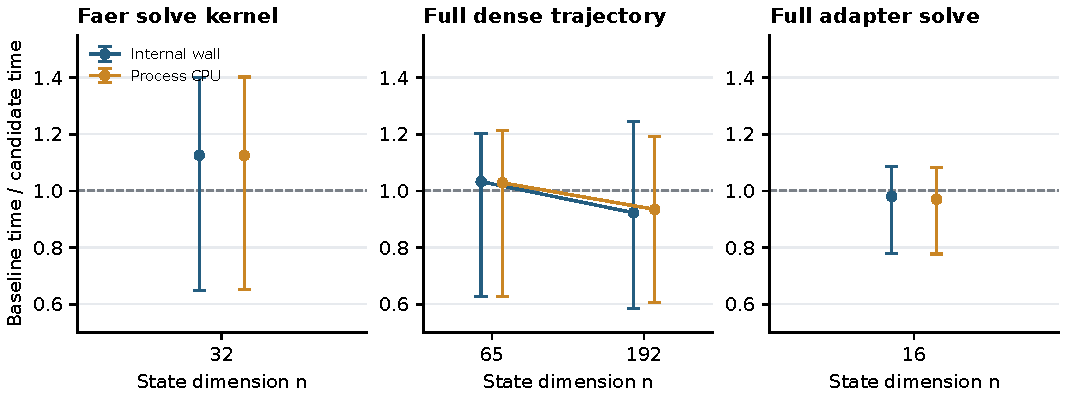
\includegraphics[width=\textwidth]{figures/performance.pdf}
\caption{Long-batch confirmation baseline/candidate time ratios. Points are medians of five
paired ABBA/BAAB block ratios; bars span the observed block minimum and maximum,
not a statistical confidence interval. Internal kernel wall time excludes
factorization. Full-solve wall intervals include setup, integration, output,
and counters. Process CPU additionally includes command warmup and serialization.
The adapter panel is a same-binary option comparison. All ranges cross unity.}
\label{fig:performance}
\end{figure*}
\begin{table*}[t]
\caption{Retained initial short-batch diagnostic timing. Values are median arm times;
speed ratios are medians of paired block ratios and need not equal the ratio
of the two displayed marginal medians. Every row passes its declared accuracy contract,
but none establishes a stable wall-time benefit.}
\label{tab:timing}
\begin{ruledtabular}
\begin{tabular}{llrrrrl}
Scope & $n$ & Baseline & Candidate & Ratio & Unit & Block-ratio range\\
\hline
LU solve & 32 & 2.128 & 1.598 & 1.074 & $\mu$s & 0.823--1.357 \\
LU solve & 96 & 10.524 & 10.357 & 1.078 & $\mu$s & 0.977--1.233 \\
LU solve & 192 & 14.895 & 14.901 & 0.996 & $\mu$s & 0.910--1.117 \\
Dense trajectory & 65 & 7.563 & 7.063 & 1.083 & ms & 0.928--1.248 \\
Dense trajectory & 96 & 16.999 & 16.960 & 1.022 & ms & 0.667--1.175 \\
Dense trajectory & 192 & 150.132 & 118.212 & 1.252 & ms & 0.844--1.598 \\
Adapter solve & 8 & 336.786 & 365.317 & 0.970 & $\mu$s & 0.859--1.099 \\
Adapter solve & 16 & 448.637 & 425.492 & 1.063 & $\mu$s & 0.945--1.095 \\
\end{tabular}
\end{ruledtabular}
\end{table*}
\begin{table}[b]
\caption{Dense trajectory accuracy on all 33 common times and all components.
All states, observation times, native counters and attempt counts are identical
in the baseline and candidate, with the same $10^{-7}$ error cap.}
\label{tab:dense-accuracy}
\begin{ruledtabular}
\begin{tabular}{lrl}
$n$ & Attempts & Maximum component error\\
\hline
65 & 81 & $4.595\times10^{-10}$ \\
96 & 81 & $4.617\times10^{-10}$ \\
192 & 81 & $4.605\times10^{-10}$ \\
\end{tabular}
\end{ruledtabular}
\end{table}
\begin{table*}[t]
\caption{Adapter work and accuracy. All accepted trajectory values are equal
between feature-off and feature-on runs. Every returned component, including
the common requested windows, meets the $10^{-5}$ cap. Work includes discarded
comparators; these reductions are not themselves time ratios.}
\label{tab:adapter-work}
\begin{ruledtabular}
\begin{tabular}{lrrrrrl}
$n$ & RHS off/on & Work off & Work on & Work reduction & Prefix wins & Maximum error\\
\hline
8 & 1120/1112 & 2119 & 2102 & 0.80\% & 1 & $6.101\times10^{-8}$ \\
16 & 1216/1200 & 2655 & 2605 & 1.88\% & 1 & $6.101\times10^{-8}$ \\
\end{tabular}
\end{ruledtabular}
\end{table*}
The sentinel-on control has identical complete trajectories and counters with
the new option off/on, as expected because the option does not change that path.
The targeted native contracts separately verify encountered-fatal priority,
conservative arithmetic near the exact-integer limit, and incomplete-evidence
semantics. The full raw records include rejected or failed build attempts as
well as successful validation. No broad historical test suite is relabeled
as a new execution.

\subsection{Negative and conditional theory results}
\begin{figure*}[t]
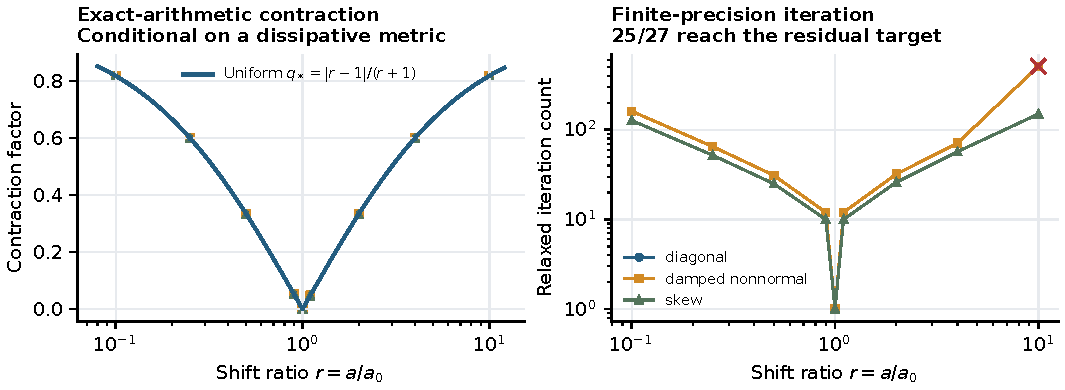
\includegraphics[width=\textwidth]{figures/theory.pdf}
\caption{Shifted-system research experiment. Left: the exact-arithmetic
uniform contraction bound and finite computed operator norms. Right: iteration
counts of the relaxed candidate. Red crosses mark two runs that reached the
512-iteration limit without attaining the unchanged $10^{-10}$ residual
threshold. Numeric norm checks are diagnostic checks, not interval certificates.}
\label{fig:theory}
\end{figure*}
\begin{table*}[t]
\caption{Selected shifted-system cells exposing both benefit and cost.
``Fail'' preserves the original stopping failure. Iteration counts are not
wall times and should not be compared as if their kernels had equal cost.}
\label{tab:theory-cells}
\begin{ruledtabular}
\begin{tabular}{llrrll}
Family & $a/a_0$ & Relaxed iterations & Unrelaxed iterations & Relaxed target & Unrelaxed target\\
\hline
diagonal & 0.1 & 161 & 44 & Pass & Fail \\
diagonal & 0.25 & 65 & 92 & Pass & Fail \\
diagonal & 4 & 71 & 61 & Pass & Pass \\
diagonal & 10 & 512 & 119 & Fail & Pass \\
damped nonnormal & 2 & 32 & 9 & Pass & Pass \\
damped nonnormal & 10 & 512 & 12 & Fail & Pass \\
skew & 1 & 1 & 1 & Pass & Pass \\
skew & 4 & 57 & 11 & Pass & Pass \\
\end{tabular}
\end{ruledtabular}
\end{table*}
The two failed relaxed residuals are approximately $4.80\times10^{-10}$ and
$4.67\times10^{-10}$, while their actual forward errors are small. This is
consistent with residual evaluation at a floating floor; it does not justify
changing the requested target after observing the failures. The new rule cures
two diagonal unrelaxed divergences but generally increases iterations elsewhere.
Consequently the theorem supplies a conditional convergence option, not an
unconditional performance replacement.


\section{What needs mathematics, and what needs engineering}
\label{sec:next}
The priority mathematical obligation is a full-domain certificate connecting a structured or projected solve to the original target. Three pieces must be bound together: (i) a model/metric/domain identity for the declared dissipativity or polynomial relation; (ii) an inverse-action defect and residual-evaluation enclosure; and (iii) the causal stage and physical-output transport, with a closed radius or tube. A sampled norm, an eigenvalue plot, or an endpoint discrepancy is insufficient for this composition. The current core already contains important pieces, including original-space residual checks, conditioned polynomial contracts, and finite causal majorants; the next work should extend and connect them, not discard them.

The shifted-factor theorem gives a concrete candidate for such an extension. It guarantees convergence in a declared dissipative metric for every positive shift ratio in exact arithmetic, but a uniform minimax rate can be much slower than the actual spectral rate of unrelaxed Richardson. The 27-cell experiment demonstrates exactly that tradeoff. A production proposal should compete with existing unrelaxed iteration, GMRES, and refactorization under the same original-target error contract. Admission requires a proved metric/drift bound and accounted floating action error. A small contraction factor alone is not a cost model.

Structural chart extensions require a similar discipline. A commuting analytic carrier can be removed exactly under its declared relation. Arbitrary noncommuting time-dependent carriers require a time-ordered evolution or a bounded surrogate defect. The chart's physical amplification and flow sensitivity must be propagated even when transformed coordinates appear benign. The V8 query-membership work is relevant evidence about a representation; it is not the missing physical enclosure itself.

The main engineering opportunities remain substantial: retained FD Jacobian and partial-time buffers; reusable JVP operator storage; persistent implicit sessions; fewer repeated losing entry pilots; rank-aware cheaper least squares; and an explicitly authorized small-system dense representation. The matrix-free cost proxy must be revised together with changes that remove diagnostic JVP counts or charge structural linear-algebra costs. Otherwise a counter reduction can make the selector's timing predictions worse. These changes should be admitted with matched outputs and actual total cost rather than a universal fixed weight fitted only to the current small examples.

This study closes the selected implementation surfaces, supplies executable mathematical prerequisites, and preserves negative results. It does not close every profiling issue, establish a universal best solver, certify arbitrary physical models, or promote the independent V8 ledger.

\appendix
\section{Reproduction and source map}
The complete packet is under \auditpath. The preregistration fixes the baseline, separate lanes, accuracy contracts, serial timing, and bounded current experiments. \code{RUN\_STATE.json} and the final manifest contain actual statuses. The report's theory body is accompanied by full prose proofs, a standalone Rust primitive, exact-CAS receipts, the 27-row numerical data, and the exact rational DOPRI derivation.

The production paths changed are \path{crates/vigilode/src/switching.rs}, \path{crates/rodas5p-core/src/matrix.rs}, its export in \path{lib.rs}, \path{crates/rodas5p-integrators/src/rodas5p_fast.rs}, \path{rodas5p_matrix_free_fast.rs}, and \path{crates/vigilode-coupled/src/residual_first.rs}. New contract tests and benchmark examples accompany them. The new evidence enum is additive and can require downstream exhaustive matches to be updated; the new public configuration field can also affect fully enumerated struct literals. The conservative incomplete-comparison predicate can change equality decisions even at ordinary counts. These are explicit API/behavior consequences, separate from the default-disabled stopping optimization.

The retained baseline binary is built from the unchanged baseline plus the same source-compatible trajectory harness. All benchmark commands are recorded, including task affinity. The resulting exact states and work counters are compared before ratios are interpreted. Reproduction on another host may change timings while preserving the algebraic and allocation conclusions.

\begin{thebibliography}{9}
\bibitem{TranquilliSandu2014} P. Tranquilli and A. Sandu, Rosenbrock--Krylov methods for large systems of differential equations, \emph{SIAM J. Sci. Comput.} \textbf{36}, A1313--A1338 (2014), \href{https://doi.org/10.1137/130923336}{doi:10.1137/130923336}, \href{https://arxiv.org/abs/1305.5481}{arXiv:1305.5481}. Primary text, Sec.~1 and Eqs.~(2a)--(2b), and joint Krylov/time-discretization order analysis.
\bibitem{LiuMoursiVanderwerff2022} L. Liu, W. M. Moursi, and J. Vanderwerff, Strongly nonexpansive mappings revisited: uniform monotonicity and operator splitting (2022), \href{https://arxiv.org/abs/2205.09040}{arXiv:2205.09040}. Primary text, Sec.~2, Fact~2.5, Eq.~(14).
\bibitem{ProfilePacket} VigilODE, Adapter profile audit, 27 October 2026, source measured at \code{46939bbe}, packet at \baseline, \path{external_reports/adapter_profile_audit_20261027/}; \href{https://github.com/cosmosapjw-quantum/vigilode/tree/3064d453091af1dec7f99f0c8afabd98b447ea34/external_reports/adapter_profile_audit_20261027}{immutable repository snapshot}. The v2 packet supersedes v1; historical wall times are diagnostic.
\bibitem{CheckpointPacket} VigilODE, Adapter checkpoint followup, 27 October 2026, \path{research/adapter_checkpoint_followup_20261027/}, baseline \code{3064d453091af1dec7f99f0c8afabd98b447ea34}.
\bibitem{IntegrationPacket} VigilODE, Adapter integration report, 27 October 2026, \path{research/adapter_integration_20261027/REPORT_KO.md}, earlier source \code{dda8d2f16758ce7d3369ad249344b2ac8bbd08ef}.
\bibitem{V8Membership} VigilODE, V8 Query Membership source and delivery, 27 October 2026. Source archive SHA-256 \path{8f8d3489dca47b2faad9b349fed586940a15383fc4794c41df9defc9d5a27a64}. Scope and limitations retained from the delivered handoff and theory record.
\bibitem{V8Tube} VigilODE, V8 Actual Tube source and delivery, 27 October 2026. Source archive SHA-256 \path{d1fe70d681dc7dfab690e1d973829997c2b4fad2bb3c70607030dc48e39506be}. No new physical campaign is asserted by this audit.
\end{thebibliography}
\end{document}
